\documentclass[12pt]{article}

% Essential packages for encoding, math, and formatting
\usepackage[utf8]{inputenc}
\usepackage[T1]{fontenc}
\usepackage{amsmath, amssymb, amsthm, mathtools, bm} % Enhanced math support
\usepackage{geometry}
\geometry{a4paper, margin=0.7in}
\usepackage{hyperref}
\hypersetup{
    colorlinks=true,
    linkcolor=blue,
    citecolor=blue,
    urlcolor=blue
}
\usepackage{microtype} % Improved typography
\usepackage{tocloft} % Table of contents customization
\usepackage{abstract} % For abstract environment
\usepackage{mathptmx} % Times-compatible math font
\usepackage{xcolor} % For colored text
\usepackage{tikz} % For mathematical diagrams
\usetikzlibrary{positioning, shapes, arrows, shadows}
\usepackage{enumitem} % Better list formatting

% Custom math commands for enhanced notation
\newcommand{\R}{\mathbb{R}}
\newcommand{\C}{\mathbb{C}}
\newcommand{\N}{\mathbb{N}}
\newcommand{\Z}{\mathbb{Z}}
\newcommand{\vect}[1]{\bm{#1}}
\newcommand{\transpose}[1]{#1^{\mathsf{T}}}
\newcommand{\norm}[1]{\left\|\,#1\,\right\|}
\newcommand{\abs}[1]{\left|\,#1\,\right|}
\newcommand{\inner}[2]{\langle\,#1,\,#2\,\rangle}

% Define theorem environments
\theoremstyle{definition}
\newtheorem{definition}{Definition}[subsection]
\newtheorem{theorem}{Theorem}[subsection]
\newtheorem{lemma}{Lemma}[subsection]
\newtheorem{proposition}{Proposition}[subsection]
\newtheorem{remark}{Remark}[subsection]

\begin{document}

% Title page
\begin{titlepage}
    \centering
    \vspace*{1cm}
    {\huge \textbf{From Projection to Perception: \\ A Mathematical Exploration of \\ Shadow-based Neural Reconstruction}\par}
    \vspace{1.5cm}
    {\normalsize
    A research report submitted to the Scientific Committee of the Hang Lung Mathematics Award\par}
    \vspace{1cm}
    {\normalsize \textbf{Team Number}\par 2596873\par}
    \vspace{0.5cm}
    {\normalsize \textbf{Team Members}\par Wong Yuk To, Hung Kwong Lam \\ Cheung Tsz Lung, Chan Ngo Tin, Zhou Lam Ho\par}
    \vspace{0.5cm}
    {\normalsize \textbf{Teacher}\par Mr. Chan Ping Ho\par}
    \vspace{0.5cm}
    {\normalsize \textbf{School}\par Po Leung Kuk Celine Ho Yam Tong College\par}
    \vspace{0.5cm}
    {\normalsize \textbf{Date}\par \today\par}
    \vspace{2cm}

% Abstract
\begin{abstract}
This paper explores \textit{ShadowNeuS} \hyperlink{[LWX23]}{[LWX23]}, a neural network that creates 3D models from single-view camera images by using clues from shadows and light. Unlike traditional methods that rely on multiple camera or sensors to build the 3D scene, \textit{ShadowNeuS} uses a neural signed distance field (SDF) to accurately reconstruct 3D geometry. We will start by understanding how the network is trained and connected to geometry with spatial reasoning in 3D space $\mathbb{R}^3$. Finally, we will check our understanding by adapting the network for 2D reconstruction using similar conditions and methods.
\end{abstract}

\end{titlepage}

% Table of contents
\tableofcontents 

\newpage
\section{Background} \label{sec:background}

\subsection{What is 3D Reconstruction from Images?} \label{sec:reconstruction_intro}

The goal of 3D reconstruction is to recover the structure of a 3D scene using only 2D images.

\begin{definition}[3D Scene Representation] \label{def:scene_repr} ~\\
A 3D scene is represented by a set of points $\vect{P} = [P_x, P_y, P_z]^\mathsf{T} \in \R^3$ in Euclidean space.
\end{definition}

\begin{definition}[Image Projection] \label{def:image_proj} ~\\
Each image $I_n$ of the 3D scene records a set of pixel coordinates $\vect{p} = [p_x, p_y]^\mathsf{T} \in \R^2$.
\end{definition}

The process of capturing a 3D point in a 2D image $I_n$ can be modeled as a projection function $\pi_n$:

\vspace{0.5em}
\begin{equation}
\boxed{\pi_n: \R^3 \to \R^2, \quad [P_x, P_y, P_z]^\mathsf{T} \mapsto [p_x, p_y]^\mathsf{T}} \label{eq:proj}
\end{equation}
\vspace{0.5em}

This projection function represents how a camera maps a 3D point to a 2D pixel in the $n$-th image.

To reconstruct the 3D scene, we need to solve the \textbf{inverse problem} $\pi_n^{-1}$:

\vspace{0.5em}
\begin{equation}
\boxed{\pi_n^{-1}(\vect{p}) = \left\{ \vect{P} \in \R^3 \mid \pi_n(\vect{P}) = \vect{p} \right\}} \label{eq:invproj}
\end{equation}
\vspace{0.5em}

However, this inverse problem is typically \textbf{ill-posed}, as multiple 3D points may project to the same 2D pixel, leading to ambiguity. We will detail this in Section \ref{sec:inverse_problem}.

\subsection{Information Encoded in 2D Images} \label{sec:image_info}

A 2D image $I_n$ can provide multiple types of information encoded as mathematical structures:

\subsubsection*{Information Available from an Image:}
\begin{enumerate}[label=(\roman*)]
    \item \textbf{Pixel coordinates}: $\vect{p} = [p_x, p_y]^\mathsf{T} \in \R^2$, represents the spatial location of each pixel
    
    \item \textbf{Color values}: $C_n(\vect{p}) = [r, g, b]^\mathsf{T} \in [0,1]^3$, represents the RGB values
    
    \item \textbf{RGB gradient matrix}:
    \begin{equation}
        \nabla C_n(\vect{p}) = \begin{bmatrix}
            \frac{\partial r}{\partial p_x} & \frac{\partial r}{\partial p_y} \\[0.5em]
            \frac{\partial g}{\partial p_x} & \frac{\partial g}{\partial p_y} \\[0.5em]
            \frac{\partial b}{\partial p_x} & \frac{\partial b}{\partial p_y}
        \end{bmatrix} \in \R^{3 \times 2} \label{eq:gradient}
    \end{equation}
    This Jacobian matrix captures local intensity variations, indicating edges or texture information.
    
    \item \textbf{Learned feature embedding}: $\phi(I_n)(\vect{p}) \in \R^d$, represents high-dimensional features extracted via neural networks like CNNs, MLPs
\end{enumerate}

These data structures result from projecting 3D geometry through camera optics, where $C_n(\vect{p})$ corresponds to visible surface and $\nabla C_n(\vect{p})$ encodes geometric boundaries.

\newpage

\subsection{The Forward Projection: From 3D World to 2D Image} \label{sec:forward_projection}

We formalize the perspective projection process using homogeneous coordinates and transformation matrices.

\subsubsection*{Camera Parameter Matrices:}

\begin{definition}[Extrinsic Parameters] \label{def:extrinsic} ~\\
The world-to-camera transformation is characterized by:
\begin{align}
\text{Camera center: } &\quad \vect{C} = [C_x, C_y, C_z]^\mathsf{T} \in \R^3 \\
\text{Rotation matrix: } &\quad R = \begin{bmatrix}
    r_{11} & r_{12} & r_{13} \\
    r_{21} & r_{22} & r_{23} \\
    r_{31} & r_{32} & r_{33}
\end{bmatrix} \in \text{SO}(3) \\
\text{Translation vector: } &\quad \vect{t} = -R \vect{C} \in \R^3
\end{align}
\end{definition}

\begin{definition}[Intrinsic Parameters] \label{def:intrinsic} ~\\
The camera's internal geometry is encoded by:
\begin{equation}
K = \begin{bmatrix}
    f_x & 0 & c_x \\
    0 & f_y & c_y \\
    0 & 0 & 1
\end{bmatrix} \in \R^{3 \times 3} \label{eq:intrinsic}
\end{equation}
where $(f_x, f_y)$ are focal lengths in pixels and $(c_x, c_y)$ is the principal point
\end{definition}

\subsubsection*{Forward Projection Pipeline:}

\begin{proposition}[Perspective Projection Transform] \label{prop:projection_pipeline} ~\\
The forward projection involves three sequential transformations of the 3D point $\vect{P}$ to pixel point $\vect{p}$:
\begin{enumerate}[label=\textbf{Step \arabic*:}]
    \item \textbf{World to camera coordinates}
    \begin{equation}
        \vect{P}_{\text{cam}} = R (\vect{P} - \vect{C}) = R \vect{P} + \vect{t}
    \end{equation}
    
    \item \textbf{Camera to image coordinates}
    \begin{equation}
        \vect{P}_{\text{hom}} = K \vect{P}_{\text{cam}} = \begin{bmatrix} p_x' \\ p_y' \\ z' \end{bmatrix}
    \end{equation}
    
    \item \textbf{Perspective division}
    \begin{equation}
        \vect{p} = \begin{bmatrix} p_x \\ p_y \end{bmatrix} = \frac{1}{z'} \begin{bmatrix} p_x' \\ p_y' \end{bmatrix}, \quad z' \neq 0
    \end{equation}
\end{enumerate}
\end{proposition}

The complete transformation matrix can be expressed as:

\vspace{0.5em}
\begin{equation}
\boxed{\vect{P}_{\text{hom}} = K [R \mid \vect{t}] \begin{bmatrix} \vect{P} \\ 1 \end{bmatrix} , \quad \vect{p} = \frac{1}{z'} \begin{bmatrix} p_x' \\ p_y' \end{bmatrix}} \label{eq:forward}
\end{equation}
\vspace{0.5em}

\newpage

\subsection{The Inverse Problem: From 2D Image to 3D World} \label{sec:inverse_problem}

We now tackle the fundamental challenge of inverting the projection function.

\begin{lemma}[Camera Ray Parametrization] \label{lem:camera_ray} ~\\
Given a pixel $\vect{p} = [p_x, p_y]^\mathsf{T}$ and camera parameters $(K, R, \vect{C})$, the corresponding 3D points form a ray:

\vspace{0.25em}
\begin{equation}
\boxed{\vect{P}(\lambda) = \vect{C} + \lambda \cdot \vect{d}, \quad \lambda > 0} \label{eq:camera_ray}
\end{equation}
\vspace{0.25em}

where the ray direction is:

\vspace{0.25em}
\begin{equation}
\boxed{\vect{d} = R^{-1} K^{-1} \begin{bmatrix} p_x \\ p_y \\ 1 \end{bmatrix}} \label{eq:ray_direction}
\end{equation}
\vspace{0.25em}
\begin{remark}[Normalization] \label{rmk:normalization} ~\\
The direction vector $\vect{d}$ can optionally be normalized to unit length for physical ray tracing but not strictly necessary for the ray parametrization.
\end{remark}
\end{lemma}

\begin{proof}
Starting from the forward projection equation \eqref{eq:forward}:
\begin{align}
K (R \vect{P} + \vect{t}) &= z' \begin{bmatrix} p_x \\ p_y \\ 1 \end{bmatrix} \\
R \vect{P} + \vect{t} &= z' K^{-1} \begin{bmatrix} p_x \\ p_y \\ 1 \end{bmatrix} \\
\vect{P} &= R^{-1} \left( z' K^{-1} \begin{bmatrix} p_x \\ p_y \\ 1 \end{bmatrix} - \vect{t} \right)
\end{align}

Since $\vect{t} = -R \vect{C}$, we have $-R^{-1} \vect{t} = \vect{C}$. Setting $\lambda = z'$:
\begin{equation}
\vect{P}(\lambda) = \vect{C} + \lambda \cdot R^{-1} K^{-1} \begin{bmatrix} p_x \\ p_y \\ 1 \end{bmatrix}
\end{equation}
\end{proof}

\begin{proposition}[Ill-posed Nature of Single-View Reconstruction] \label{prop:illposed} ~\\
The inverse projection problem is fundamentally \textbf{ill-posed} because:
\begin{enumerate}[label=(\alph*)]
    \item The depth parameter $\lambda$ is undetermined
    \item Each pixel $\vect{p}$ defines a ray of infinitely many possible 3D points
    \item Additional constraints are required for unique reconstruction
\end{enumerate}
\end{proposition}

\newpage

\subsection{Cues for Solving the Inverse Problem} \label{sec:cues}

To achieve unique reconstruction, we require additional information such as:
\begin{itemize}
    \item \textbf{Stereo correspondence}: Multiple viewpoints providing triangulation
    \item \textbf{Depth sensors}: Direct measurement of $\lambda$
    \item \textbf{Shadow constraints}: Geometric relationships via light-surface interactions
\end{itemize}

\section{Shadows as a Geometric Constraint} \label{sec:shadows}

To what extent can shadows constrain 3D geometry from a single image? In this section, we formalize shadow formation, analyze the geometric information it provides, discuss its limitations and set up the motivation for neural solutions.

\subsection{Light Ray and Shadow Geometry} \label{sec:light_ray_geometry}

\begin{definition}[Light Ray] \label{def:light_ray} ~\\
Given a point light source $\vect{L} \in \R^3$ and a surface point $\vect{P} \in \R^3$, the light ray is:
\begin{equation}
\boxed{r(t) = \vect{L} + t(\vect{P} - \vect{L}), \quad t \in [0,1]} \label{eq:light_ray}
\end{equation}
\end{definition}

\begin{definition}[Shadow Occlusion Test] \label{def:shadow_occlusion} ~\\
A point $\vect{P}$ is in shadow if there exists $t \in (0,1)$ such that the light ray intersects a surface $\mathcal{S}$:
\begin{equation}
\boxed{r(t) \cap \mathcal{S} \neq \emptyset, \quad t \in (0,1)}
\end{equation}
\end{definition}

\begin{remark}[Physical Interpretation] \label{rmk:occlusion_physics} ~\\
The interval $(0,1)$ excludes the light source ($t=0$) and the target point ($t=1$), ensuring the test checks for obstructions between $\vect{L}$ and $\vect{P}$. This models physical light transport where occlusion by another surface causes a shadow.
\end{remark}

\subsection{Shadow Boundary and Surface Partitioning} \label{sec:shadow_boundary}

\begin{theorem}[Tangency Condition] \label{thm:tangency} ~\\
A point $\vect{Q} \in \mathcal{S}$ lies on the shadow boundary if and only if the light direction is tangent to the surface:
\begin{equation}
\boxed{(\vect{Q} - \vect{L}) \cdot \vect{n}(\vect{Q}) = 0} \label{eq:tangency}
\end{equation}
where $\vect{n}(\vect{Q})$ is the outward unit normal at $\vect{Q}$.
\end{theorem}

\begin{proof}
At the shadow boundary, the light ray $r(t)$ grazes the surface $\mathcal{S}$ at $\vect{Q}$, meaning the direction $\vect{Q} - \vect{L}$ lies in the tangent plane. Thus, it is perpendicular to the surface normal $\vect{n}(\vect{Q})$,  $(\vect{Q} - \vect{L}) \cdot \vect{n}(\vect{Q}) = 0$.
\end{proof}

\begin{definition}[Shadow Boundary Set] \label{def:boundary_set} ~\\
The 3D shadow boundary is:
\begin{equation}
\boxed{\mathcal{B} = \{\vect{Q} \in \mathcal{S} \mid (\vect{Q} - \vect{L}) \cdot \vect{n}(\vect{Q}) = 0\}} \label{eq:boundary_set}
\end{equation}
\end{definition}

\newpage

\begin{proposition}[Surface Illumination Partition] \label{prop:illumination_partition} ~\\
The surface $\mathcal{S}$ is partitioned into three disjoint regions based on the light direction:
\begin{align}
\mathcal{S}_{\text{lit}} &= \{\vect{P} \in \mathcal{S} \mid (\vect{P} - \vect{L}) \cdot \vect{n}(\vect{P}) < 0\} && \text{(illuminated)} \label{eq:lit_region} \\
\mathcal{S}_{\text{shadow}} &= \{\vect{P} \in \mathcal{S} \mid (\vect{P} - \vect{L}) \cdot \vect{n}(\vect{P}) > 0\} && \text{(attached shadow)} \label{eq:shadow_region} \\
\mathcal{B} &= \{\vect{P} \in \mathcal{S} \mid (\vect{P} - \vect{L}) \cdot \vect{n}(\vect{P}) = 0\} && \text{(shadow boundary)} \label{eq:boundary_region}
\end{align}
\end{proposition}

\begin{remark}[Geometric Interpretation] \label{rmk:illum_sign} ~\\
The sign of $(\vect{P} - \vect{L}) \cdot \vect{n}(\vect{P})$ reflects the angle between the light direction and the surface normal, determining whether a point is lit, shadowed, or on the boundary.
\end{remark}

\subsection{Cast Shadow Regions} \label{sec:cast_shadow}

\begin{definition}[Cast Shadow Region] \label{def:cast_shadow} ~\\
For an occluding surface $\mathcal{S}_1$ and a receiving surface $\mathcal{S}_2$, the cast shadow region is:
\begin{equation}
\boxed{\mathcal{C}_{1 \to 2} = \{\vect{P} \in \mathcal{S}_2 \mid \exists t \in (0,1): \vect{L} + t(\vect{P} - \vect{L}) \in \mathcal{S}_1\}} \label{eq:cast_shadow}
\end{equation}
\end{definition}

\begin{remark}[Cast Shadow Formation] \label{rmk:cast_shadow_formation} ~\\
A point $\vect{P} \in \mathcal{S}_2$ is in the cast shadow if the light ray from $\vect{L}$ to $\vect{P}$ is blocked by $\mathcal{S}_1$. For multiple occluders $\mathcal{S}_1, \mathcal{S}_2, \ldots, \mathcal{S}_k$, a point is shadowed if it lies in $\bigcup_{i=1}^k \mathcal{C}_{i \to \text{target}}$. Self-shadowing occurs when $\mathcal{S}_1 = \mathcal{S}_2$, as a surface may occlude itself.
\end{remark}

\begin{definition}[Cast Shadow Boundary] \label{def:cast_boundary} ~\\
The cast shadow boundary on $\mathcal{S}_2$ is:
\begin{equation}
\boxed{\partial\mathcal{C}_{1 \to 2} = \{\vect{P} \in \mathcal{S}_2 \mid \vect{P} = \vect{Q} + s(\vect{Q} - \vect{L}), \vect{Q} \in \mathcal{B}_1, s > 0\}} \label{eq:cast_boundary}
\end{equation}
where $\mathcal{B}_1$ is the shadow boundary on $\mathcal{S}_1$ (Equation \eqref{eq:boundary_set}).
\end{definition}

\begin{proposition}[Multi-Surface Cast Shadows and Boundaries] \label{prop:multi_cast} ~\\
For $k$ occluders, the total cast shadow region and its boundary on a target surface are:
\begin{equation}
\boxed{\mathcal{C}_{\text{total}} = \bigcup_{i=1}^k \mathcal{C}_{i \to \text{target}} \label{eq:total_cast_region}}
\end{equation}
\begin{equation}
\boxed{\partial\mathcal{C}_{\text{total}} = \partial (\bigcup_{i=1}^k \mathcal{C}_{i \to \text{target}}) \label{eq:total_cast_boundary}}
\end{equation}
where $\mathcal{C}_{i \to \text{target}}$ is the cast shadow region from $\mathcal{S}_i$ and $\partial\mathcal{C}_{i \to \text{target}}$ is its boundary.
\end{proposition}

\subsection{Shadow Regions in Images} \label{sec:shadow_in_image}

\begin{definition}[Image Shadow and Lit Regions] \label{def:image_shadow_regions} ~\\
Given the projection function $\pi: \mathbb{R}^3 \to \mathbb{R}^2$ (Equation \eqref{eq:proj}), the image $I$ is partitioned as:
\begin{align}
\Omega_{\text{lit}}^{\text{obs}} &= \{\pi(\vect{P}) \mid \vect{P} \in \mathcal{S}_{\text{lit}}, \pi(\vect{P}) \text{ not occluded}\} && \text{(lit region)} \label{eq:image_lit} \\
\Omega_{\text{shadow}}^{\text{obs}} &= \{\pi(\vect{P}) \mid \vect{P} \in \mathcal{S}_{\text{shadow}} \cup \mathcal{C}_{\text{total}}, \pi(\vect{P}) \text{ not occluded}\} && \text{(shadow region)} \label{eq:image_shadow} \\
\partial\Omega_{\text{shadow}}^{\text{obs}} &= \{\pi(\vect{P}) \mid \vect{P} \in \mathcal{B} \cup \partial\mathcal{C}_{\text{total}}, \pi(\vect{P}) \text{ not occluded}\} && \text{(shadow boundary)} \label{eq:image_boundary}
\end{align}
where $\mathcal{S}_{\text{lit}}$, $\mathcal{S}_{\text{shadow}}$, $\mathcal{B}$, and $\mathcal{C}_{\text{total}}$ are defined in Equations \eqref{eq:lit_region}, \eqref{eq:shadow_region}, \eqref{eq:boundary_region}, and \eqref{eq:total_cast_region}. Only points not occluded by the object contribute to $\Omega_{\text{shadow}}^{\text{obs}}$, as shadows may be blocked by the object itself.
\end{definition}

\begin{remark}[Shadow Projection and Occlusion] \label{rmk:shadow_projection} ~\\
The projection $\pi$ maps 3D points to 2D image pixels. A lit point $\vect{P} \in \mathcal{S}_{\text{lit}}$ projects to a bright pixel $\pi(\vect{P}) \in \Omega_{\text{lit}}^{\text{obs}}$ if not occluded by the object. Similarly, a shadowed point $\vect{P} \in \mathcal{S}_{\text{shadow}} \cup \mathcal{C}_{\text{total}}$ projects to a dark pixel in $\Omega_{\text{shadow}}^{\text{obs}}$ only if not occluded. Shadows cast by the object may be hidden, so not all shadowed points appear in the image.
\end{remark}

\begin{definition}[Shadow Region Classification Accuracy] \label{def:shadow_accuracy} ~\\
This accuracy metric evaluates how well the reconstructed 3D geometry correctly predicts the image regions classified as lit, shadowed, or the boundary:
\begin{equation}
\text{Accuracy} = \frac{\text{Number of correctly predicted pixels}}{\text{Total number of pixels}} = \frac{N_{\text{correct}}}{N_{\text{total}}}
\end{equation}
\end{definition}

\subsection{Shadows as Cues for 3D Reconstruction} \label{sec:shadow_cues}

\subsubsection*{Geometric Information Encoded in Shadows} \label{sec:shadow_geom_info}

Shadows provide critical geometric constraints for single-view 3D reconstruction, leveraging light-surface interactions.
= 
\begin{proposition}[Shadow-Derived Geometric Cues] \label{prop:shadow_cues} ~\\
From observed shadows, we can infer:
\begin{enumerate}[label=(\roman*)]
    \item \textbf{Surface Orientation:} Points in attached shadows satisfy
    \[
    (\vect{P} - \vect{L}) \cdot \vect{n}(\vect{P}) > 0
    \]
    as in Equation~\eqref{eq:shadow_region}, indicating that the surface at $\vect{P}$ is facing away from the light source.

    \item \textbf{Tangency Constraints at Boundaries:} For points on the shadow boundary, the incoming light direction lies in the surface's tangent plane:
    \[
    (\vect{Q} - \vect{L}) \cdot \vect{n}(\vect{Q}) = 0
    \]
    (Equation~\eqref{eq:tangency}). This geometric constraint localizes the transition between lit and shadowed regions.

    \item \textbf{Relative Depth from Cast Shadows:} If $\vect{P} \in \mathcal{C}_{1 \to 2}$ (cast shadow region), then the occluding surface $\mathcal{S}_1$ must be geometrically in front of $\mathcal{S}_2$ along the light direction, as defined in Equation~\eqref{eq:cast_shadow}. This gives ordinal depth information.

    \item \textbf{Occlusion Structure:} The presence of a shadow implies the existence of an occluder blocking the light ray from $\vect{L}$ to $\vect{P}$, indicating some intermediate geometry between the light and the shadowed surface point.
\end{enumerate}
\end{proposition}

\begin{remark}[Depth Ordering via Cast Shadows] \label{rmk:depth_order} ~\\
Cast shadows provide explicit ordering information. If a point $\vect{P}$ on surface $\mathcal{S}_2$ is shadowed due to surface $\mathcal{S}_1$, then $\mathcal{S}_1$ must lie between the light source $\vect{L}$ and $\vect{P}$ along the ray. This insight can be directly encoded into optimization or inference schemes.
\end{remark}

\newpage

\subsubsection*{Shadow Depth Recovery} \label{sec:shadow_depth}

For a pixel $\vect{p}$ on the shadow boundary, depth recovery combines the camera ray (\ref{eq:camera_ray}) with the Surface Illumination Partition (\ref{prop:illumination_partition}):

\begin{equation}
\boxed{
\begin{aligned}
\vect{P}(\lambda) &= \vect{C} + \lambda \vect{d} \quad \text{and} \quad
\begin{cases}
(\vect{P}(\lambda) - \vect{L}) \cdot \hat{\vect{n}} > 0 \\[6pt]
(\vect{P}(\lambda) - \vect{L}) \cdot \hat{\vect{n}} = 0 \\[6pt]
(\vect{P}(\lambda) - \vect{L}) \cdot \hat{\vect{n}} < 0
\end{cases}
\end{aligned}
}
\label{eq:shadow_depth_system}
\end{equation}

\begin{theorem}[Depth from Shadow] \label{thm:shadow_depth} ~\\
Given surface normal estimate \(\hat{\vect{n}}\), the depth parameter \(\lambda\) satisfies:
\begin{equation}
\boxed{
\begin{cases}
\lambda > \displaystyle \frac{(\vect{L} - \vect{C}) \cdot \hat{\vect{n}}}{\vect{d} \cdot \hat{\vect{n}}} & \text{(in attached shadow region)} \\[8pt]
\lambda = \displaystyle \frac{(\vect{L} - \vect{C}) \cdot \hat{\vect{n}}}{\vect{d} \cdot \hat{\vect{n}}} & \text{(on shadow boundary)} \\[8pt]
\lambda < \displaystyle \frac{(\vect{L} - \vect{C}) \cdot \hat{\vect{n}}}{\vect{d} \cdot \hat{\vect{n}}} & \text{(point is illuminated)}
\end{cases}
}
\label{eq:lambda_solution}
\end{equation}
where \(\vect{d} \cdot \hat{\vect{n}} \neq 0\).
\end{theorem}

\subsubsection*{Limitations and Computational Challenges} \label{sec:shadow_limitations}

\paragraph{Fundamental Challenges}
\begin{enumerate}[label=\arabic*.]
    \item \textbf{Circular Dependency:} Equation~\eqref{eq:lambda_solution} requires surface normals $\hat{\vect{n}}$ at point $P(\lambda)$ to find the value of $\lambda$.
    
    \item \textbf{Singular Cases:} Solution undefined when $\vect{d} \cdot \hat{\vect{n}} = 0$ (grazing angles).
    
    \item \textbf{Non-Unique Solutions:} Multiple depth values may satisfy shadow conditions for complex surfaces.
\end{enumerate}

\paragraph{Computational Challenges}
\begin{enumerate}[label=\arabic*., resume]
    \item \textbf{Non-Differentiable Occlusion:} The condition $r(t) \cap \mathcal{S} \neq \emptyset$ prevents gradient-based optimization. This discrete intersection test returns binary values (occluded/not occluded) with undefined gradients at surface boundaries, making automatic differentiation impossible.
    
    \item \textbf{Nonlinear Systems:} Equation~\eqref{eq:shadow_depth_system} requires iterative solvers with convergence issues.
    
    \item \textbf{Ray Tracing Complexity:} Cast shadow computation scales as $O(n^2)$ for $n$ surface points. Each of the $n$ points requires testing occlusion against all other $n-1$ potential occluders, yielding $n(n-1) = O(n^2)$ ray-surface intersection tests.
\end{enumerate}

\paragraph{Practical Issues}
\begin{enumerate}[label=\arabic*., resume]
    \item \textbf{Light Localization:} Unknown light position $\vect{L}$ must be estimated, introducing error propagation.
    
    \item \textbf{Shadow Detection:} Real images have soft shadows, noise, and ambient lighting that blur the shadow information.
    
    \item \textbf{Multi-Object Complexity:} Overlapping shadows from multiple objects complicate the total cast region $\mathcal{C}_{\text{total}}$.
\end{enumerate}

\newpage

\begin{remark}[Neural Solutions] \label{rmk:neural_solutions} ~\\
Modern neural approaches address classical limitations through the following key advances:

\begin{center}
\begin{tabular}{|l|p{5.5cm}|p{5.5cm}|}
\hline
\textbf{Challenge} & \textbf{Classical Limitation} & \textbf{Neural Solution} \\
\hline
\textbf{Differentiability} & Binary occlusion tests block gradient flow & Differentiable functions enable backpropagation through entire pipeline \\
\hline
\textbf{Circular Dependencies} & Needs normals to compute depth, needs depth to compute normals & Implicit surfaces (SDF/NeRF) represent geometry and normals jointly \\
\hline
\textbf{Computational Efficiency} & O(n²) ray tracing for cast shadows & Parallel GPU processing, learned approximations \\
\hline
\textbf{Robustness} & Fails on soft shadows, noise, complex lighting & Handles real-world imperfections through learned representations \\
\hline
\textbf{Integration} & Separate modules for lighting, geometry, materials & Unified model learns all components simultaneously \\
\hline
\end{tabular}
\end{center}

These methods transform geometric constraints into trainable optimization objectives, bridging classical shadow analysis with neural reconstruction.
\end{remark}

\section{ShadowNeuS: Neural Shadow-Based 3D Reconstruction} \label{sec:shadowneus}

ShadowNeuS addresses single-view 3D reconstruction under specific controlled conditions:

\begin{itemize}
    \item \textbf{Single camera viewpoint}: Fixed camera position and orientation.
    \item \textbf{Multiple lighting conditions}: Images captured under a set of known light source positions $\{\mathbf{L}_i\}$.
    \item \textbf{Calibrated light positions}: Light source locations are known or pre-calibrated.
    \item \textbf{Static scene}: No object movement between lighting conditions.
    \item \textbf{Observable shadows}: Clear and distinguishable shadow boundaries in the captured images.
\end{itemize}

This setup allows ShadowNeuS to leverage shadow cues to recover complete 3D geometry, including occluded or non-visible regions, by combining classical geometric reasoning with neural optimization.

\subsection{Classical vs Neural Approaches: Method Comparison} \label{sec:method_comparison}

Figures~\ref{fig:classical_method} and~\ref{fig:neural_method} illustrate the processing pipelines for classical geometric methods and ShadowNeuS respectively.

\begin{figure}[htbp]
\centering
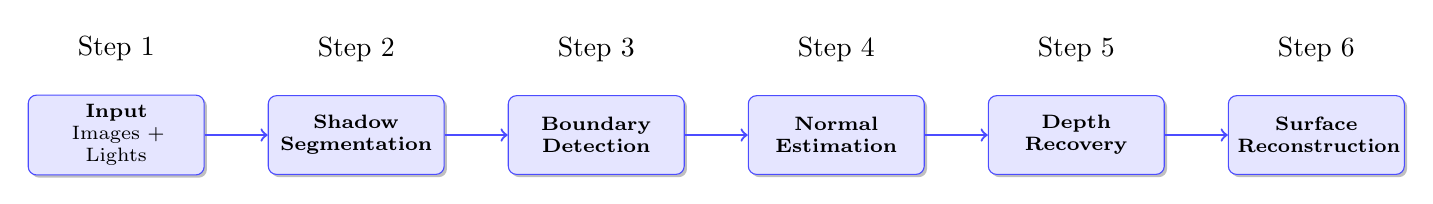
\begin{tikzpicture}[
    node distance=0.8cm,
    classicalbox/.style={rectangle, draw=blue!70, fill=blue!10, rounded corners=3pt, 
                        text width=2cm, text centered, minimum height=1cm, font=\scriptsize,
                        drop shadow={shadow xshift=1pt, shadow yshift=-1pt}},
    arrow/.style={->, thick, blue!70}
]

\node[classicalbox] (input) {\textbf{Input} \\ Images + Lights};
\node[classicalbox, right=of input] (shadow_seg) {\textbf{Shadow} \\ \textbf{Segmentation}};
\node[classicalbox, right=of shadow_seg] (boundary_det) {\textbf{Boundary} \\ \textbf{Detection}};
\node[classicalbox, right=of boundary_det] (normal_est) {\textbf{Normal} \\ \textbf{Estimation}};
\node[classicalbox, right=of normal_est] (depth_solve) {\textbf{Depth} \\ \textbf{Recovery}};
\node[classicalbox, right=of depth_solve] (surface_recon) {\textbf{Surface} \\ \textbf{Reconstruction}};

\draw[arrow] (input) -- (shadow_seg);
\draw[arrow] (shadow_seg) -- (boundary_det);
\draw[arrow] (boundary_det) -- (normal_est);
\draw[arrow] (normal_est) -- (depth_solve);
\draw[arrow] (depth_solve) -- (surface_recon);


% Timeline
\node[above=0.3cm of input] {Step 1};
\node[above=0.3cm of shadow_seg] {Step 2};
\node[above=0.3cm of boundary_det] {Step 3};
\node[above=0.3cm of normal_est] {Step 4};
\node[above=0.3cm of depth_solve] {Step 5};
\node[above=0.3cm of surface_recon] {Step 6};

\end{tikzpicture}
\caption{Classical method (Sequential processing pipeline)}
\label{fig:classical_method}
\end{figure}

\begin{figure}[htbp]
\centering
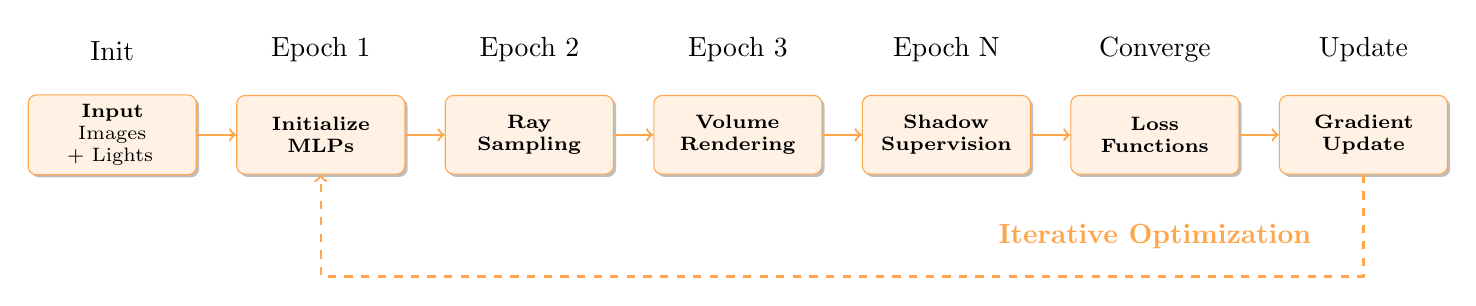
\begin{tikzpicture}[
    node distance=0.5cm,
    neuralbox/.style={rectangle, draw=orange!70, fill=orange!10, rounded corners=3pt,
                     text width=1.9cm, text centered, minimum height=1cm, font=\scriptsize,
                     drop shadow={shadow xshift=1pt, shadow yshift=-1pt}},
    arrow/.style={->, thick, orange!70},
]

\node[neuralbox] (input) {\textbf{Input} \\ Images + Lights};
\node[neuralbox, right=of input] (init_mlp) {\textbf{Initialize} \\ \textbf{MLPs}};
\node[neuralbox, right=of init_mlp] (ray_sample) {\textbf{Ray} \\ \textbf{Sampling}};
\node[neuralbox, right=of ray_sample] (volume_render) {\textbf{Volume} \\ \textbf{Rendering}};
\node[neuralbox, right=of volume_render] (shadow_super) {\textbf{Shadow} \\ \textbf{Supervision}};
\node[neuralbox, right=of shadow_super] (loss_compute) {\textbf{Loss} \\ \textbf{Functions}};
\node[neuralbox, right=of loss_compute] (gradient_update) {\textbf{Gradient} \\ \textbf{Update}};

\draw[arrow] (input) -- (init_mlp);
\draw[arrow] (init_mlp) -- (ray_sample);
\draw[arrow] (ray_sample) -- (volume_render);
\draw[arrow] (volume_render) -- (shadow_super);
\draw[arrow] (shadow_super) -- (loss_compute);
\draw[arrow] (loss_compute) -- (gradient_update);

\draw[arrow, dashed] (gradient_update) -- ++(0,-1.8) -| (init_mlp);
\node[below=of loss_compute, text=orange!70] {\textbf{Iterative Optimization}};

% Timeline
\node[above=0.3cm of input] {Init};
\node[above=0.3cm of init_mlp] {Epoch 1};
\node[above=0.3cm of ray_sample] {Epoch 2};
\node[above=0.3cm of volume_render] {Epoch 3};
\node[above=0.3cm of shadow_super] {Epoch N};
\node[above=0.3cm of loss_compute] {Converge};
\node[above=0.3cm of gradient_update] {Update};

\end{tikzpicture}
\caption{ShadowNeuS (End-to-end neural optimization pipeline)}
\label{fig:neural_method}
\end{figure}

\subsection{ShadowNeuS Pipeline} \label{sec:classical_to_neural}

In this section, we outline the complete pipeline of ShadowNeuS, from the initialization of neural SDFs to optimization using shadow supervision.

\subsubsection{Neural Signed Distance Fields (SDF)} \label{sec:neural_sdf}

\begin{definition}[Neural Signed Distance Field] \label{def:neural_sdf} ~\\
A \textbf{Neural Signed Distance Field} (Neural SDF), as introduced in \hyperlink{[PFS19]}{[PFS19]}, is a function $f(\mathbf{P}; \theta): \mathbb{R}^3 \to \mathbb{R}$ parameterized by a multi-layer perceptron (MLP) with trainable weights $\theta$. It implicitly represents a 3D scene by outputting the signed distance of any spatial point $\mathbf{P} = (p_x, p_y, p_z)^\top$ to the nearest surface:
\[
f(\mathbf{P}) =
\begin{cases}
< 0 & \text{if } \mathbf{P} \text{ is inside the object}, \\
= 0 & \text{if } \mathbf{P} \text{ lies on the surface}, \\
> 0 & \text{if } \mathbf{P} \text{ is outside the object}.
\end{cases}
\]
\end{definition}

\begin{remark}[Key Mathematical Properties of Neural SDF] \label{rmk:gradient_properties} ~\\
Neural SDFs encode geometric and differential properties useful for 3D reconstruction from shadow cues:
\begin{itemize}

    \item \textbf{Differentiability}: $f(\mathbf{P}; \theta)$ is differentiable with respect to both spatial coordinates $\mathbf{P}$ and neural parameters $\theta$, enabling end-to-end gradient-based optimization:
    \[
    \nabla_{\mathbf{P}} f(\mathbf{P}; \theta), \quad \nabla_{\theta} f(\mathbf{P}; \theta).
    \]
    
    \item \textbf{Surface Normals}: At the zero-level set $f(\mathbf{P}) = 0$, the unit surface normal vector is computed via normalized spatial gradients:
    \begin{equation}
    \hat{\mathbf{n}}(\mathbf{P}) = \frac{\nabla_{\mathbf{P}} f(\mathbf{P})}{\|\nabla_{\mathbf{P}} f(\mathbf{P})\|_2}. \label{eq:sdf_normal}
    \end{equation}
    This facilitates shadow-based light visibility computations via the angle between $\hat{\mathbf{n}}$ and the light direction $\mathbf{L} - \mathbf{P}$.

    \item \textbf{Eikonal Regularization (Distance Consistency)}: For $f(\mathbf{P})$ to represent a valid distance function locally, it must satisfy the \textit{Eikonal equation}:
    \begin{equation}
    \|\nabla_{\mathbf{P}} f(\mathbf{P})\|_2 = 1, \quad \forall \mathbf{P} \in \mathbb{R}^3. \label{eq:eikonal_constraint}
    \end{equation}
    A first-order Taylor approximation confirms this property:
    \begin{equation}
    f(\mathbf{P} + \sigma \mathbf{u}) \approx f(\mathbf{P}) + \sigma \cdot \left( \nabla_{\mathbf{P}} f(\mathbf{P}) \cdot \mathbf{u} \right), \quad \|\mathbf{u}\|_2 = 1, |\sigma| \ll 1. \label{eq:taylor_sdf_property}
    \end{equation}

    \item \textbf{Geometric Stability}: Deviations from $\|\nabla_{\mathbf{P}} f(\mathbf{P})\|_2 = 1$ indicate distortion:
    \[
    \|\nabla_{\mathbf{P}} f(\mathbf{P})\|_2
    \begin{cases}
    > 1 & \text{implies local stretching (distance overestimation)}, \\
    < 1 & \text{implies local compression (distance underestimation)}.
    \end{cases}
    \]
    Enforcing the Eikonal constraint regularizes the SDF, ensuring stable and consistent geometry during optimization.
    
\end{itemize}
\end{remark}

\subsubsection{Epoch 1: Neural SDF Initialization and MLP Design} \label{sec:epoch1_neural_sdf}

The training begins by constructing a neural signed distance field (SDF), modeled by an eight-layer multi-layer perceptron (MLP) to implicitly represent 3D geometry from shadow cues. 

\begin{itemize}

    \item \textbf{Network Structure}: ShadowNeuS uses an 8-layer fully-connected MLP with ReLU activation functions, a single output head producing scalar signed distances $f(\mathbf{P}; \theta) \in \mathbb{R}$.

    \begin{remark}[Why MLP Architecture?] ~\\
    The MLP design offers several advantages:
    \begin{itemize}
        \item \textbf{Universal Approximation}: By the universal approximation theorem, MLPs can approximate any continuous function on compact subsets of $\mathbb{R}^3$.
        \item \textbf{End-to-End Differentiability}: Gradients $\nabla_{\mathbf{P}} f$, $\nabla_{\theta} f$ can be computed throughout the pipeline, enabling training directly from shadow observations.
        \item \textbf{Joint Integrative Learning}: Both surface positions ($f(\mathbf{P}) = 0$) and surface normals ($\nabla_{\mathbf{P}} f$) are jointly encoded in $f$, simplifying the learning process compared to classical pipelines which handle these separately.
        \item \textbf{Circular Dependency Resolution}: Neural SDF jointly models geometry and visibility, avoiding the iterative or circular inversion problems faced by classical shadow methods.
    \end{itemize}
    \end{remark}

    \item \textbf{Input Encoding}: To enhance the ability of the MLP to capture high-frequency geometric features, ShadowNeuS applies a sinusoidal positional encoding $\gamma(\mathbf{P})$ to the input 3D coordinates:
    \begin{equation}
    \gamma(\mathbf{P}) = \left( \sin(2^0 \pi p_x), \cos(2^0 \pi p_x), \ldots, \sin(2^{k-1} \pi p_z), \cos(2^{k-1} \pi p_z) \right).
    \end{equation}

    \begin{remark}[Why Positional Encoding?] ~\\
    Raw coordinates $\mathbf{P} = (p_x, p_y, p_z)$ do not provide sufficient high-frequency variation for MLPs, leading to overly smooth approximations (spectral bias). Positional encoding introduces Fourier feature mappings \hyperlink{[TSS20]}{[TSS20]}, allowing the network to represent both coarse and fine geometric structures revealed by shadows.
    \end{remark}

    \item \textbf{Output}: A scalar SDF value $f(\mathbf{P})$ per point.

    \item \textbf{Random Initialization}: The MLP weights $\theta$ are initialized using standard techniques such as Xavier initialization, ensuring well-scaled activations in early epochs.
\end{itemize}

\subsubsection{Epoch 2$\to$N: Ray Sampling and Shadow Rendering} \label{sec:epoch2_ray_sampling}

From the second epoch onward, ShadowNeuS iteratively performs \textbf{ray sampling} to locate surface points and \textbf{shadow rendering} to predict shadow values at image pixels. The procedure proceeds as follows:

\begin{itemize}

    \item \textbf{Camera Ray Sampling}: \\
    For each pixel $\mathbf{p}$, a camera ray is constructed:
    \[
    \mathbf{r}(t) = \mathbf{C} + t \mathbf{d}, \quad \mathbf{d} = R^{-1} K^{-1} \begin{bmatrix} p_x \\ p_y \\ 1 \end{bmatrix}.
    \]
    The intersection point $\mathbf{P}$ is found by sphere tracing along $\mathbf{r}(t)$ to locate $t^*$ satisfying
    \[
    f_\theta(\mathbf{r}(t^*)) = 0, \quad \mathbf{P} = \mathbf{r}(t^*).
    \]

    \item \textbf{Light Ray Sampling and Visibility Estimation}: \\
    For each $\mathbf{P}$, a light ray towards the light source $\mathbf{L}$ is defined:
    \[
    \mathbf{l}(s) = \mathbf{P} + s (\mathbf{L} - \mathbf{P}), \quad s \in [0, 1].
    \]
    The \textbf{opacity} along $\mathbf{l}(s)$ is computed at discrete points $\mathbf{l}(s_j)$ using:
    \[
    a_j = \max\left( 1 - \frac{ \phi(f_\theta(\mathbf{l}(s_{j+1})) ) }{ \phi(f_\theta(\mathbf{l}(s_j))) }, 0 \right)
    \]
    where $\phi(\cdot)$ is an active function, and $a_j \in [0,1]$ represents the \textbf{local opacity} between adjacent samples.

    The accumulated transmittance (incoming light intensity) is then:
    \[
    C_{\mathrm{in}}(\mathbf{P}) = \prod_{j=1}^N (1 - a_j)
    \]
    This idea is inspired by Neural Radiance Fields (NeRF) \hyperlink{[MST20]}{[MST20]}, which uses volume rendering to synthesize views from radiance fields.
\end{itemize}

\subsubsection{Converge: Loss Functions} \label{sec:loss_functions}

The overall objective of the training process is to minimize a weighted sum of several loss terms that enforce both geometric and appearance-based constraints. The total loss function is defined as:
\begin{equation}
\mathcal{L}_{\text{total}} = w_{\text{shadow}} \cdot \mathcal{L}_{\text{shadow}} + w_{\text{eik}} \cdot \mathcal{L}_{\text{eik}} + w_{\text{app}} \cdot \mathcal{L}_{\text{appearance}} + \ldots
\end{equation}

\begin{itemize}
    \item \textbf{Shadow Supervision Loss:}
    \begin{equation}
    \mathcal{L}_{\text{shadow}} = \sum_{\mathbf{p}} \left| C_{\mathrm{in}}(\mathbf{p}) - S(\mathbf{p}) \right|
    \end{equation}
    This term measures the difference between the predicted incoming light intensity $C_{\mathrm{in}}(\mathbf{p})$ and the observed shadow value $S(\mathbf{p})$ over all valid image pixels $\mathbf{p}$.

    \item \textbf{Eikonal Loss:}
    \begin{equation}
    \mathcal{L}_{\text{eik}} = \frac{1}{M} \sum_{i=1}^M \left( \left\| \nabla f(\mathbf{P}_i) \right\|_2 - 1 \right)^2
    \end{equation}
    This regularization ensures the predicted signed distance function (SDF) $f$ has unit gradient norm almost everywhere, encouraging smooth and well-defined surfaces.

    \item \textbf{Appearance or Consistency Loss:}
    \begin{equation}
    \mathcal{L}_{\text{appearance}} = \sum_{\mathbf{p}} \left\| C_{\text{pred}}(\mathbf{p}) - C_{\text{gt}}(\mathbf{p}) \right\|_2^2
    \end{equation}
    This term enforces color or texture consistency by minimizing the error between predicted colors $C_{\text{pred}}$ and ground-truth colors $C_{\text{gt}}$ at pixel locations $\mathbf{p}$. Depending on the dataset, it can also include feature or texture-based losses.

    \item \textbf{Other Loss Terms (optional):}
    
    Additional loss terms such as normal supervision, depth alignment, or regularization losses can be added when extra supervision signals are available.
\end{itemize}

\newpage

\subsubsection{Gradient Descent and Adam Optimizer} \label{sec:adam_optimizer}

To minimize the total loss $\mathcal{L}_{\text{total}}(\theta)$, neural networks typically rely on gradient-based optimization methods. Below, we summarize both the basic gradient descent method and the more advanced Adam optimizer used in our implementation. Details of Adam optimizer are refered to paper \hyperlink{[KB14]}{[KB14]}.

\begin{itemize}

    \item \textbf{Gradient Descent}: The simplest optimization method updates the parameters $\theta$ along the direction of steepest descent, defined by the negative gradient of the loss:
    \[
    \theta_{t+1} = \theta_t - \alpha \, \nabla_\theta \mathcal{L}_{\text{total}}(\theta_t),
    \]
    where $\theta_t$ denotes the parameters at iteration $t$, $\alpha > 0$ is the \textbf{learning rate}, and $\nabla_\theta \mathcal{L}_{\text{total}}$ is the gradient of the total loss with respect to $\theta$.

    \begin{remark}[Limitations of Simple Gradient Descent]
    Despite its simplicity, basic gradient descent exhibits several limitations:
    \begin{itemize}
        \item \textbf{Learning Rate Sensitivity}: A fixed $\alpha$ may result in slow convergence (if too small) or divergence (if too large).
        \item \textbf{Oscillation}: In regions with steep or curved loss landscapes, updates can oscillate and hinder convergence.
        \item \textbf{Uniform Step Size}: All parameters are updated using the same learning rate, without accounting for variations in gradient magnitude.
    \end{itemize}
    \end{remark}

    \item \textbf{Adam Optimizer}: Adaptive Moment Estimation (Adam) addresses these issues by combining:
    \begin{itemize}
        \item \textbf{Momentum (First Moment Estimate)}: Adam maintains an exponentially decaying average of past gradients:
        \[
        m_t = \beta_1 m_{t-1} + (1 - \beta_1) g_t, \quad g_t = \nabla_\theta \mathcal{L}_{\text{total}}(\theta_t),
        \]
        where $0 < \beta_1 < 1$ controls the momentum decay. This term reduces oscillations and stabilizes updates.

        \item \textbf{Adaptive Scaling (Second Moment Estimate)}: Adam also tracks the exponentially decaying average of squared gradients:
        \[
        v_t = \beta_2 v_{t-1} + (1 - \beta_2) g_t^2,
        \]
        where $0 < \beta_2 < 1$ governs the decay rate for squared gradients. This adjusts learning rates per parameter based on historical gradient magnitudes.

        \item \textbf{Bias Correction}: To correct for initialization bias (since $m_0, v_0 = 0$), Adam computes bias-corrected estimates:
        \[
        \hat{m}_t = \frac{m_t}{1 - \beta_1^t}, \quad \hat{v}_t = \frac{v_t}{1 - \beta_2^t}.
        \]
    \end{itemize}

    \item \textbf{Adam Update Rule}: The final parameter update rule is given by:
    \[
    \theta_{t+1} = \theta_t - \alpha \cdot \frac{\hat{m}_t}{\sqrt{\hat{v}_t} + \epsilon},
    \]
    where:
    \begin{itemize}
        \item $\alpha$ is the learning rate (e.g., $\alpha = 10^{-3}$),
        \item $\beta_1$ is the first moment decay rate (typically $\beta_1 = 0.9$),
        \item $\beta_2$ is the second moment decay rate (typically $\beta_2 = 0.999$),
        \item $\epsilon$ is a small constant (e.g., $\epsilon = 10^{-8}$) to ensure numerical stability and prevent division by zero.
    \end{itemize}

\end{itemize}

\newpage

%%%%%%%%%%%%%%%%%%%%%%%%%%%%%%%%%%%%%%%%%%%%%%%

% \section{1D Shadow-Based Reconstruction Experiment} \label{sec:1d_experiment}

% \subsection{Problem Formulation: 2D Reconstruction from 1D Observations} \label{sec:1d_problem}

% \subsubsection*{Dimensional Reduction of ShadowNeuS} \label{sec:dimensional_reduction}

% % Content: Reducing 3D→2D problem to 2D→1D, mathematical simplification

% \subsubsection*{1D Shadow Projection Model} \label{sec:1d_projection}

% % Content: 1D camera model, light source, shadow formation in 2D→1D setting

% \subsubsection*{Mathematical Framework} \label{sec:1d_framework}

% % Content: 1D SDF, ray equations, shadow constraints in reduced dimension

% \subsection{Experimental Setup} \label{sec:experimental_setup}

% \subsubsection*{Synthetic 2D Scene Generation} \label{sec:2d_scene_gen}

% % Content: Creating test scenes, ground truth 2D shapes, lighting setup

% \subsubsection*{1D Shadow Profile Creation} \label{sec:1d_profile}

% % Content: Projecting 2D scenes to 1D observations, shadow profile extraction

% \subsubsection*{Network Architecture Design} \label{sec:1d_network}

% % Content: Simplified neural network for 1D→2D reconstruction, architectural choices

% \subsection{Implementation and Results} \label{sec:implementation_results}

% \subsubsection*{Training Protocol} \label{sec:training_protocol}

% % Content: Training procedure, hyperparameters, convergence criteria

% \subsubsection*{Reconstruction Quality Metrics} \label{sec:quality_metrics}

% % Content: Evaluation metrics, comparison with ground truth, quantitative results

% \subsubsection*{Comparison with Classical Methods} \label{sec:classical_comparison}

% % Content: Baseline comparisons, advantages of neural approach

% \subsection{Analysis and Insights} \label{sec:analysis_insights}

% \subsubsection*{Convergence Behavior} \label{sec:convergence_analysis}

% % Content: Training dynamics, loss evolution, stability analysis

% \subsubsection*{Shadow Constraint Effectiveness} \label{sec:shadow_effectiveness}

% % Content: Ablation studies, impact of shadow supervision

% \subsubsection*{Limitations and Future Directions} \label{sec:limitations_future}

% % Content: Current limitations, potential improvements, scaling to higher dimensions

\newpage

\section*{References}
\begin{tabular}{@{}p{0.15\textwidth} p{0.85\textwidth}}
\hypertarget{[LWX23]}{[LWX23]} & Jingwang Ling, Zhibo Wang, Feng Xu. \textit{ShadowNeuS: Neural SDF Reconstruction by Shadow Ray Supervision}. arXiv: \href{https://arxiv.org/abs/2211.14086}{2211.14086}, 2023. \\
\hypertarget{[PFS19]}{[PFS19]} & Jeong Joon Park, Peter Florence, Julian Straub, Richard Newcombe, Steven Lovegrove. \textit{DeepSDF: Learning Continuous Signed Distance Functions for Shape Representation}. arXiv: \href{https://arxiv.org/abs/1901.05103}{1901.05103}, 2019. \\
\hypertarget{[TSS20]}{[TSS20]} & Matthew Tancik, Pratul P. Srinivasan, Ben Mildenhall, Sara Fridovich-Keil, Nithin Raghavan, Utkarsh Singhal, Ravi Ramamoorthi, Jonathan T. Barron, Ren Ng. \textit{Fourier Features Let Networks Learn High Frequency Functions in Low Dimensional Domains}. arXiv: \href{https://arxiv.org/abs/2006.10739}{2006.10739}, 2020. \\
\hypertarget{[MST20]}{[MST20]} & Ben Mildenhall, Pratul P. Srinivasan, Matthew Tancik, Jonathan T. Barron, Ravi Ramamoorthi, Ren Ng. \textit{NeRF: Representing Scenes as Neural Radiance Fields for View Synthesis}. arXiv: \href{https://arxiv.org/abs/2003.08934}{2003.08934}, 2020. \\
\hypertarget{[KB14]}{[KB14]} & Diederik P. Kingma, Jimmy Ba. \textit{Adam: A Method for Stochastic Optimization}. arXiv: \href{https://arxiv.org/abs/1412.6980}{1412.6980}, 2014.

\end{tabular}

\end{document}
